% questions.tex —— 1977 年·陕西卷 · 题目内容片段（无答案）
% 由 tools/generate_projects.py 依来源总账自 1977/1977_数学真题_陕西_试题.md 生成，勿手改（改源 MD 后重跑）


\gkpart{数学试题解（陕西卷）}

\begin{gktip}
\textbf{来源说明}：本题面依据固定源 PDF《陕西1977年高考数学试题解》第 1—7 页（书籍页码 112—117）逐题转录，解答依据同一 PDF 核对。固定源是题面与解答连续出现的试题解合排材料，不是无答案试卷；正式题为第一至第十题共 10 道，末尾“参考题”两道不计入题量。原卷不分文理、无附加题，各题不标分值；扫描件第 1 页顶部带有相邻页透印的镜像文字，非本卷内容。
\end{gktip}

\par\medskip

\begin{question}
\gkti{1}求值：

\nopagebreak[4]
\[
\left(\frac{1}{300}\right)^{-\frac12}
+10\left(\frac{\sqrt3}{2}\right)^{\frac12}\cdot\left(\frac{27}{4}\right)^{\frac14}
-10(2-\sqrt3)^{-1}.
\]

\end{question}
\begin{question}
\gkti{2}求值：$\sin480^\circ\cdot\cos480^\circ\cdot\cos960^\circ\cdot\cos1920^\circ$。

\end{question}
\begin{question}
\gkti{3}化简：$|6-a|-|2a+1|+\sqrt{a^2+10a+25}$（$a<-5$）。

\end{question}
\begin{question}
\gkti{4}解不等式：$\lg(2x+1)>\lg(5-x)$。

\end{question}
\begin{question}
\gkti{5}设 $A\text{、}B$ 为锐角，且 $\sin A=\dfrac35$，$\sin B=\dfrac5{13}$，求 $\operatorname{tg}(A-B)$。

\end{question}
\begin{question}
\gkti{6}实数 $p\text{、}q$ 应满足怎样的条件，才能使方程 $x^2+px+q=0$ 的两根成为一直角三角形两锐角的正弦？

\Needspace{0.4\textheight}
\end{question}
\begin{question}
\gkti{7}以任意一点到已知三角形三个顶点连线的中点为顶点作三角形。所作三角形的面积是已知三角形的几倍？

\begin{gktip}
原源 PDF 第 3 页解答处附有点 $P$ 与 $\triangle ABC$ 及中点三角形 $A'B'C'$ 的示意图；LaTeX 版按源图重绘。
\end{gktip}
\nopagebreak[4]
\begin{center}% 1977 年陕西卷第七题：P 为 △ABC 外一点，A′、B′、C′ 分别为 PA、PB、PC 的中点，
% 虚线为中点三角形 A′B′C′（按源卷第 3 页布局：P 左上、A 右上、B 左下、C 右下，C 带实心点）
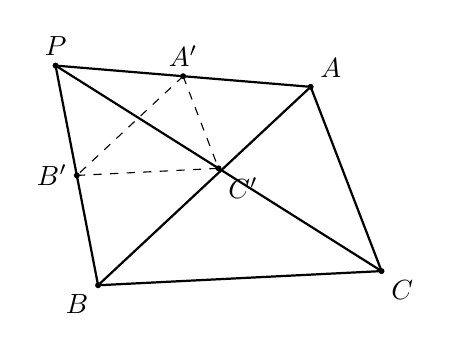
\begin{tikzpicture}[scale=0.9]
  \coordinate (P)  at (0,3.1);
  \coordinate (A)  at (3.6,2.8);
  \coordinate (B)  at (0.6,0);
  \coordinate (C)  at (4.6,0.2);
  \coordinate (Ap) at (1.8,2.95);
  \coordinate (Bp) at (0.3,1.55);
  \coordinate (Cp) at (2.3,1.65);
  \draw[thick] (P)--(A);
  \draw[thick] (P)--(B);
  \draw[thick] (P)--(C);
  \draw[thick] (A)--(B);
  \draw[thick] (B)--(C);
  \draw[thick] (A)--(C);
  \draw[dashed] (Ap)--(Bp);
  \draw[dashed] (Bp)--(Cp);
  \draw[dashed] (Ap)--(Cp);
  \fill (P)  circle (1.2pt) node[above] {$P$};
  \fill (A)  circle (1.2pt) node[above right] {$A$};
  \fill (B)  circle (1.2pt) node[below left] {$B$};
  \fill (C)  circle (1.2pt) node[below right] {$C$};
  \fill (Ap) circle (1.2pt) node[above] {$A'$};
  \fill (Bp) circle (1.2pt) node[left] {$B'$};
  \fill (Cp) circle (1.2pt) node[below right] {$C'$};
\end{tikzpicture}
\end{center}
\nopagebreak[4]
\end{question}
\begin{question}
\gkti{8}求过椭圆 $\dfrac{x^2}{13^2}+\dfrac{y^2}{12^2}=1$ 的右侧的焦点，且与圆 $x^2+y^2=3^2$ 相切的直线方程。

\end{question}
\begin{question}
\gkti{9}三角形的一内角为 $30^\circ$，它的一邻边长为 $4$，对边长为 $\dfrac52$，求另一边长。

\Needspace{0.4\textheight}
\end{question}
\begin{question}
\gkti{10}在一块边长为 $a$ 的正方形上，切着两边截去了一个半径为 $r$ 的圆料（$r\leqslant\dfrac{(2-\sqrt2)a}{4}$），如果象图 1 那样截出一个正方形的料，它的面积为多大？如果象图 2 那样截出的一个正方形的料，它的面积为多大？这二种截法截下的正方形的料的面积哪个较大？

\begin{gktip}
原源 PDF 第 5 页解答处附有图 1、图 2 两幅示意图；LaTeX 版按源图重绘。
\end{gktip}
\nopagebreak[4]
\begin{center}% 1977 年陕西卷第十题图 1：正方形 ABCD 的角 B 处切着两边截去半径为 r 的圆料，
% 截出的正方形 A′B′C′D 与原正方形共角 D，顶点 B′ 落在对角线 BD 与圆的交点处（按源卷第 5 页布局）
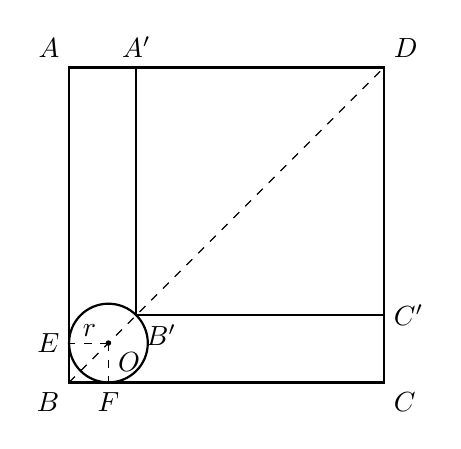
\begin{tikzpicture}[scale=1.0]
  \draw[thick] (0,0)--(4,0)--(4,4)--(0,4)--cycle;
  \draw[thick] (0.8536,4)--(0.8536,0.8536);
  \draw[thick] (0.8536,0.8536)--(4,0.8536);
  \draw[thick] (0.5,0.5) circle (0.5);
  \draw[dashed] (0,0)--(4,4);
  \draw[dashed] (0.5,0.5)--(0,0.5);
  \draw[dashed] (0.5,0.5)--(0.5,0);
  \fill (0.5,0.5) circle (1pt) node[below right] {$O$};
  \node at (0.26,0.66) {$r$};
  \node[left]  at (0,0.5)   {$E$};
  \node[below] at (0.5,0)   {$F$};
  \node[above left]  at (0,4)      {$A$};
  \node[above]       at (0.8536,4) {$A'$};
  \node[above right] at (4,4)      {$D$};
  \node[right]  at (4,0.8536) {$C'$};
  \node[below right] at (4,0)      {$C$};
  \node[below left]  at (0,0)      {$B$};
  \node[below right] at (0.8536,0.8536) {$B'$};
\end{tikzpicture}
\end{center}
\nopagebreak[4]
\nopagebreak[4]
\begin{center}% 1977 年陕西卷第十题图 2：圆与两边 AB、BC 相切于 E、F，且与内接正方形 A′B′C′D′ 的边 A′B′ 相切于 G
% （顶点标注按解答正文用 D′；源图该点印作 D，撇号系描图脱落）
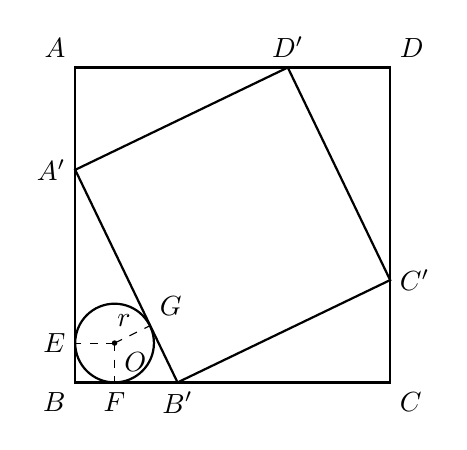
\begin{tikzpicture}[scale=1.0]
  \draw[thick] (0,0)--(4,0)--(4,4)--(0,4)--cycle;
  \draw[thick] (0,2.7)--(1.3,0)--(4,1.3)--(2.7,4)--cycle;
  \draw[thick] (0.5,0.5) circle (0.5);
  \draw[dashed] (0.5,0.5)--(0,0.5);
  \draw[dashed] (0.5,0.5)--(0.5,0);
  \draw[dashed] (0.5,0.5)--(0.95,0.72);
  \fill (0.5,0.5) circle (1pt) node[below right] {$O$};
  \node at (0.62,0.78) {$r$};
  \node[above right] at (0.95,0.72) {$G$};
  \node[left]  at (0,0.5) {$E$};
  \node[below] at (0.5,0) {$F$};
  \node[above left]  at (0,4)    {$A$};
  \node[left]        at (0,2.7)  {$A'$};
  \node[above]       at (2.7,4)  {$D'$};
  \node[above right] at (4,4)    {$D$};
  \node[right]       at (4,1.3)  {$C'$};
  \node[below left]  at (0,0)    {$B$};
  \node[below]       at (1.3,0)  {$B'$};
  \node[below right] at (4,0)    {$C$};
\end{tikzpicture}
\end{center}
\nopagebreak[4]
\textbf{参考题 1．} 在一个椭圆的所有内接矩形中，怎样的矩形面积最大？

\begin{gktip}
原源 PDF 第 6 页解答处附有椭圆与内接矩形的示意图；LaTeX 版按源图重绘。
\end{gktip}
\nopagebreak[4]
\begin{center}% 1977 年陕西卷参考题一：椭圆 x^2/a^2 + y^2/b^2 = 1 的内接矩形 ABCD，
% 长 AD=2x、宽 CD 为纵弦，x 轴标 ±a、y 轴标 ±b（按源卷第 6 页布局）
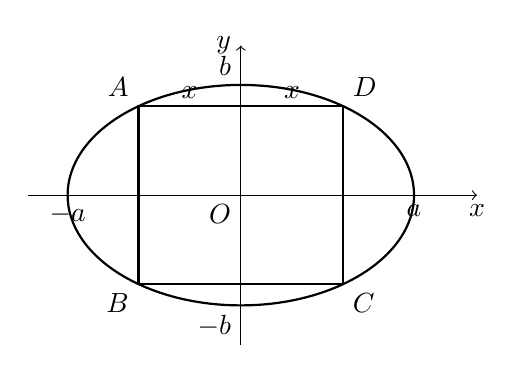
\begin{tikzpicture}[scale=1.0]
  \draw[->] (-2.7,0)--(3.0,0) node[below] {$x$};
  \draw[->] (0,-1.9)--(0,1.9) node[left] {$y$};
  \draw[thick] (0,0) ellipse (2.2 and 1.4);
  \draw[thick] (-1.3,-1.13) rectangle (1.3,1.13);
  \node[above left]  at (-1.3,1.13)  {$A$};
  \node[above right] at (1.3,1.13)   {$D$};
  \node[below left]  at (-1.3,-1.13) {$B$};
  \node[below right] at (1.3,-1.13)  {$C$};
  \node at (-0.65,1.3) {$x$};
  \node at (0.65,1.3)  {$x$};
  \node[below left]  at (0,0)     {$O$};
  \node[below]       at (-2.2,0)  {$-a$};
  \node[below]       at (2.2,0)   {$a$};
  \node[above left]  at (0,1.4)   {$b$};
  \node[below left]  at (0,-1.4)  {$-b$};
\end{tikzpicture}
\end{center}
\nopagebreak[4]
\Needspace{5\baselineskip}
\textbf{参考题 2．} 试解

\nopagebreak[4]
\[
\frac{dy}{dx}-2xy=2x^3,
\qquad
y\Big|_{x=0}=1.
\]

\end{question}